\chapter{有意识和无意识的心理过程障碍} \label{chap:chap59}

尽管认知神经科学作为一门重要的新学科出现于 20 世纪末,但术语认知的确切含义仍然难以捉摸。
该术语在不同的上下文中以不同的方式使用。
在一个极端,认知神经科学中的术语认知意味着旧术语信息处理的含义。
从这个意义上说,认知就是大脑所做的事情。
当认知神经科学家说视觉特征或运动行为由神经活动表示时,他们使用的是来自信息处理的概念。
从这个角度来看,认知语言在神经活动和行为的描述之间架起了一座桥梁,因为相同的术语可以应用于这两个领域。


在另一个极端,术语认知指的是那些对意识体验的形成至关重要的更高层次的过程。
这就是术语认知疗法的含义,这是一种由亚伦贝克和阿尔伯特埃利斯开创并从行为疗法发展而来的治疗方法。
认知疗法不是试图直接改变患者的行为,而是旨在改变患者的态度和信念(方框 59-1)。


在通常的说法中,术语认知意味着思考和推理,一种更接近其拉丁词根 cognoscere(了解或感知)的用法。
因此,《牛津英语词典》将其定义为“认识的行动或能力”。
事实上,我们通过对感官的原始数据进行思考和推理来了解世界。


这个想法隐含在我们对多种认知障碍的描述中。
脑损伤后,一些患者无法再处理感官提供的输入。
这种类型的障碍首先由西格蒙德·弗洛伊德 (Sigmund Freud) 描述,他称之为失认症或知识丧失(第 \ref{chap:chap59} 章)。
失认症可以有多种形式。
视觉失认症患者可以看得很清楚,但不再能够识别或理解他所看到的东西。
患有面部失认症的患者在识别面孔方面存在特殊问题。
患有听觉失认症的患者可能听得很好,但无法识别口语。


认知有时从出生就受损,因此一个人很难获得知识。
这可能会导致一般智力低下,或者,如果问题更局限,会导致特定的学习困难,例如阅读障碍(难以学习书面语言)或自闭症(难以了解其他思想)。
最后,认知会变得功能失调,以至于获得的关于世界的知识是错误的。
这些思维障碍导致与精神分裂症等主要精神疾病相关的错误观念(幻觉)和错误信念(妄想)。



\section{有意识和无意识的认知过程具有不同的神经相关性}

认知——通过思考和推理获得知识——是意识的三个组成部分之一(见第 \ref{chap:chap42} 章对情绪的意识方面的讨论,通常称为感受)。
另外两个是情感和意志。
过去人们理所当然地认为,思考和推理是在有意识的自愿控制下进行的,没有意识就不可能有认知。
然而,到 19 世纪末,弗洛伊德发展了一种无意识心理过程理论,并提出许多人类行为是由我们不知道的内部过程引导的。


对神经科学更直接重要的是无意识推理的概念,它最初是由亥姆霍兹提出的。
亥姆霍兹是第一个进行定量心理物理学实验并测量周围神经传入信号传导速度的人。
在这些实验之前,人们假设感觉信号会立即(以光速)到达大脑,但亥姆霍兹表明神经传导实际上非常缓慢。
他还指出,反应时间甚至更慢。
这些观察表明,大量的大脑工作介入了感官刺激和对物体的有意识感知之间。
亥姆霍兹得出结论,大脑中发生的大部分事情都不是有意识的,进入意识的东西(即被感知的东西)取决于无意识的推论。
换句话说,大脑使用来自感官的证据来决定最有可能引起感觉器官活动的物体的身份,但这是在我们没有意识到的情况下进行的。


这种观点在亥姆霍兹的同时代人中极为不受欢迎,事实上,今天仍然如此。
大多数人认为,意识是进行推理所必需的,道德责任只能分配给基于有意识推理的决定。
如果可以在没有意识的情况下进行推论,那么就没有赞扬或责备的伦理基础。
亥姆霍兹关于无意识推理的观点在很大程度上被忽视了。


尽管如此,到 20 世纪中叶,越来越多的证据支持大多数认知过程从未进入意识的观点。
随着电子计算机的发展和人工智能研究的出现,研究人员开始研究机器如何以及在多大程度上感知超越自身的世界。


尽管如此,到 20 世纪中叶,越来越多的证据支持大多数认知过程从未进入意识的观点。
随着电子计算机的发展和人工智能研究的出现,研究人员开始研究机器如何以及在多大程度上感知超越自身的世界。
很快就很清楚,许多乍一看很简单的感知过程在定义为一组计算时实际上非常复杂。


视觉感知是最好的例子。
在 1960 年代,几乎没有人意识到制造能够识别物体形状和外观的机器有多么困难,因为这对我们来说似乎太容易了。
我看着窗外,看到建筑物、树木、花朵和人。
我不知道这种看法背后有任何心理过程;
我对所有这些对象的意识似乎是瞬间和直接的。
事实证明,在包含许多重叠对象的典型杂乱视觉场景中,教机器如何计算出哪些边缘与哪个对象对应是非常困难的。
视觉的计算方法揭示了我们对世界看似毫不费力的感知所依赖的潜在神经过程。
类似的过程是所有感官知觉的基础,尤其是将声音感知为语音的基础。
大多数神经科学家现在认为,我们没有意识到认知过程,只有我们的知觉。


无意识认知过程的证据不仅来自人工智能研究,还来自脑损伤患者的认知研究。
无意识过程对行为的影响可以在某些“盲视”患者身上得到最显着的证明,这是劳伦斯·维斯克兰茨 (Lawrence Weiskrantz) 在 1970 年代首次描述的一种疾病。 这些患者的初级视觉皮层有病变,并声称在受损区域的视野部分看不到任何东西。
然而,当被要求猜测时,他们能够检测到简单的视觉属性,例如运动或颜色,这比偶然预期的要好得多。
尽管在视野的盲区对物体没有基于感官的感知,但这些患者确实拥有关于物体的无意识信息,并且这些信息可用于指导他们的行为。


另一个例子是右顶叶病变引起的单侧忽视(第 \ref{chap:chap17} 章)。
患有这种疾病的患者视力正常,但他们似乎没有注意到前方空间左侧的物体。
有些患者甚至忽略了左侧的个别物体。
在 John Marshall 和 Peter Halligan 的一项实验中,向患者展示了两幅房屋的图纸。
一所房子的左侧着火了(图 \ref{fig:59_1})。 当被问及房子之间是否有任何差异时,患者回答“没有”。 但当被问及他们更愿意住在哪所房子时,他们选择了没有着火的房子。 因此,这种选择是基于意识中未表示的信息做出的。 盲视和单方面忽视只是无意识认知过程存在的丰富经验证据的两个例子,我们无法通过内省获得这些证据。

\begin{figure}[htbp]
	\centering
	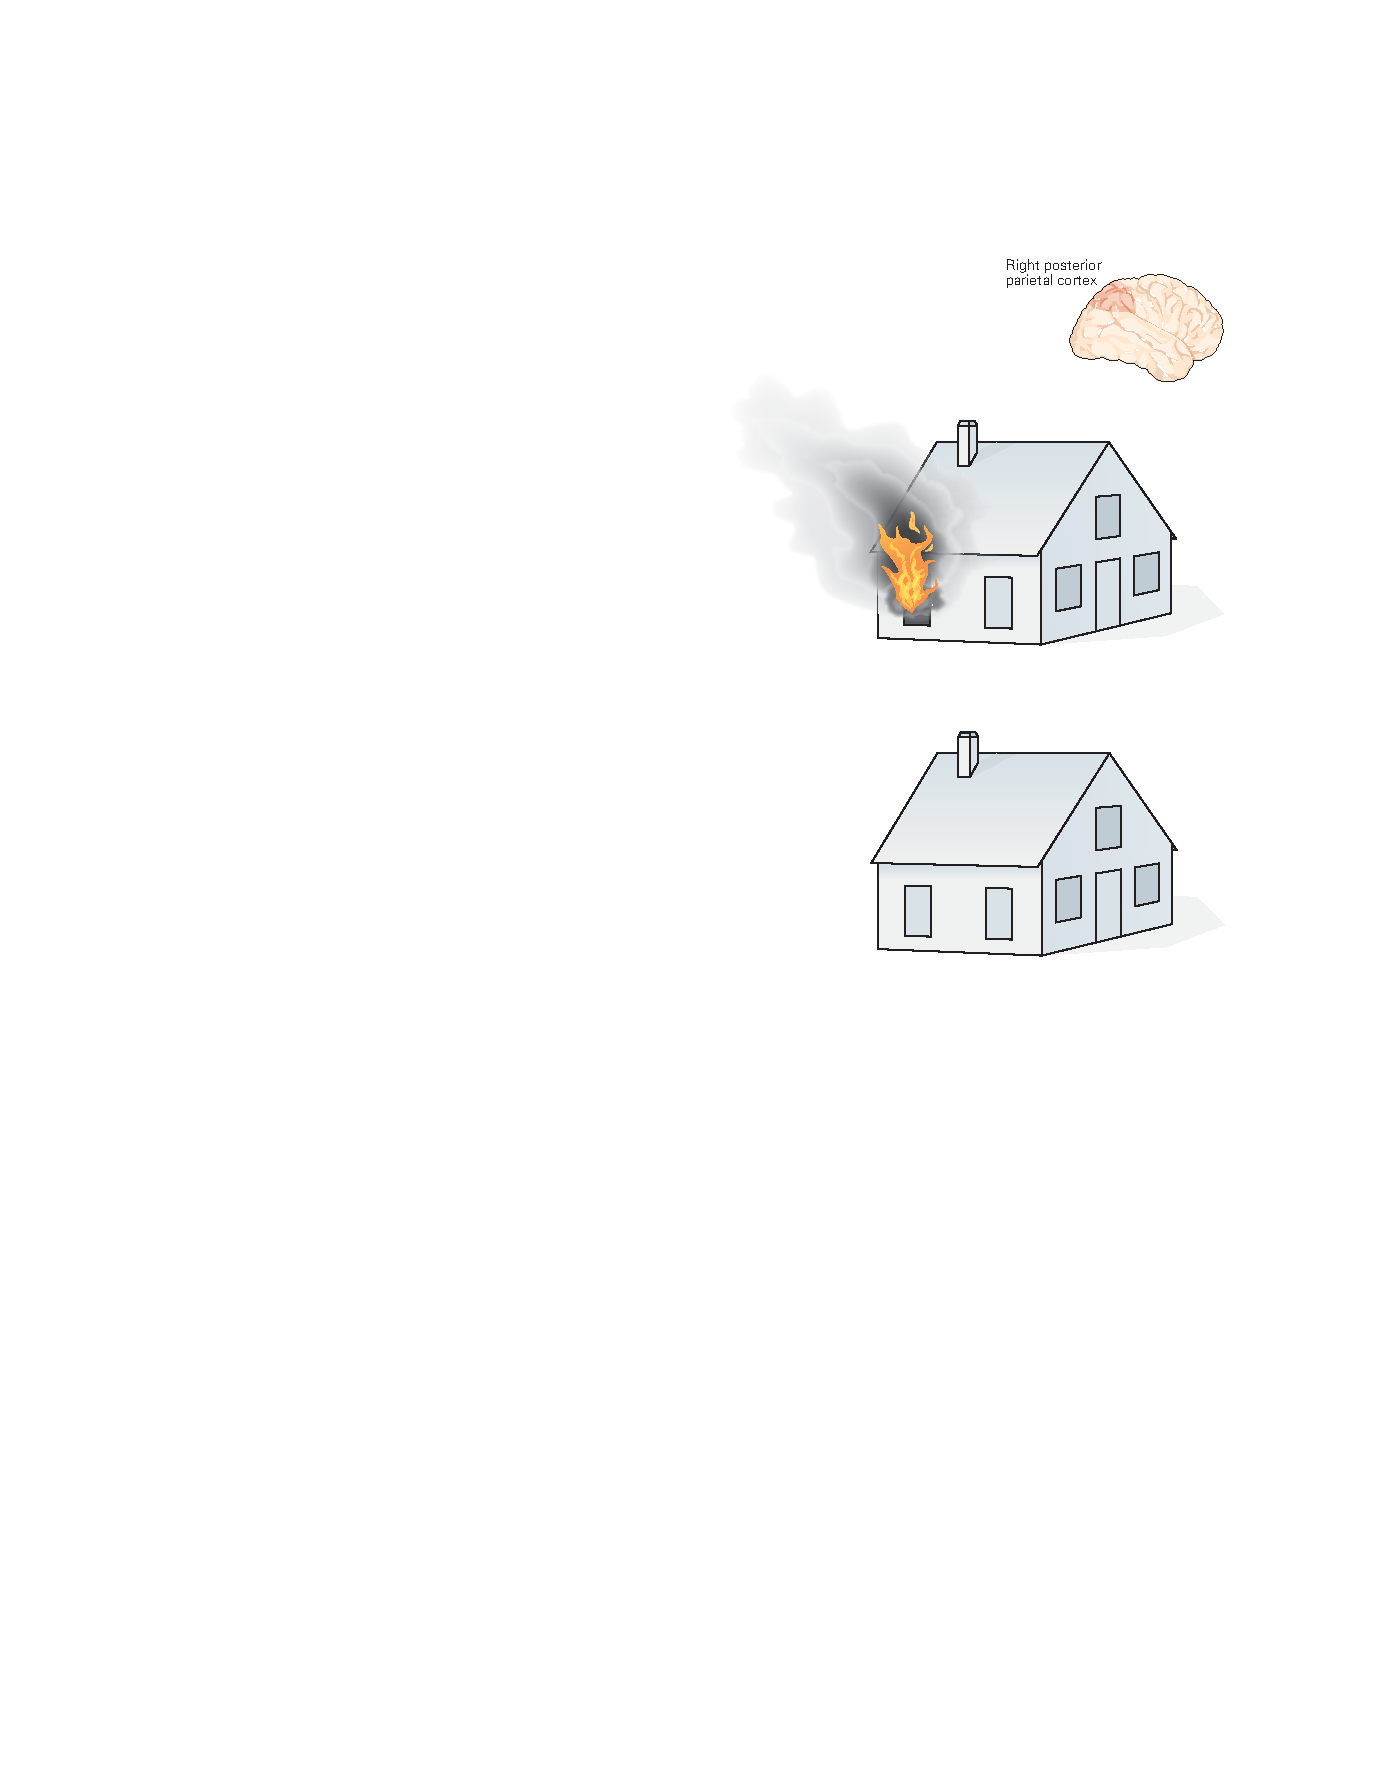
\includegraphics[width=0.5\linewidth]{chap59/fig_59_1}
	\caption{空间忽视情况下的无意识处理。 右顶叶受损后,许多患者似乎意识不到左侧空间(单侧忽视综合征)。 当这些患者看到这里复制的两幅图时,他们说这两座房子看起来一样。 然而,他们也表示他们更愿意住在下层房子里,这表明他们已经不自觉地处理了另一栋房子发生火灾的形象。 (改编自 Marshall 和 Halligan 1988。)}
	\label{fig:59_1}
\end{figure}

目前,神经科学最令人兴奋的研究领域之一是寻找由 Francis Crick 和 Christopher Koch 发起的意识的神经关联。
目的是证明与有意识和无意识认知过程相关的神经活动之间的定性差异。
这项研究很重要,不仅因为它可以为我们解答意识功能这一难题,还因为它与我们对许多神经和精神疾病的理解有关。
患有某些认知障碍的患者的怪异经历和妄想信念曾一度被认为无法理解而被忽视。
认知神经科学为我们提供了一个框架来理解这些经验和信念是如何从正常认知机制的特定改变中产生的。



\section{在脑损伤后可以以夸张的形式看到感知过程中的有意识和无意识过程之间的差异}

感官刺激和知觉之间的关系远非直接的。
知觉可以在感觉刺激没有任何变化的情况下发生变化,如鲁宾图和内克立方体等模棱两可的图所示(图 \ref{fig:59_2})。
相反,在观察者没有意识到这种变化的情况下,感官刺激可能会发生巨大变化——感知保持不变。
一个令人信服的例子是变化失明。


\begin{figure}[htbp]
	\centering
	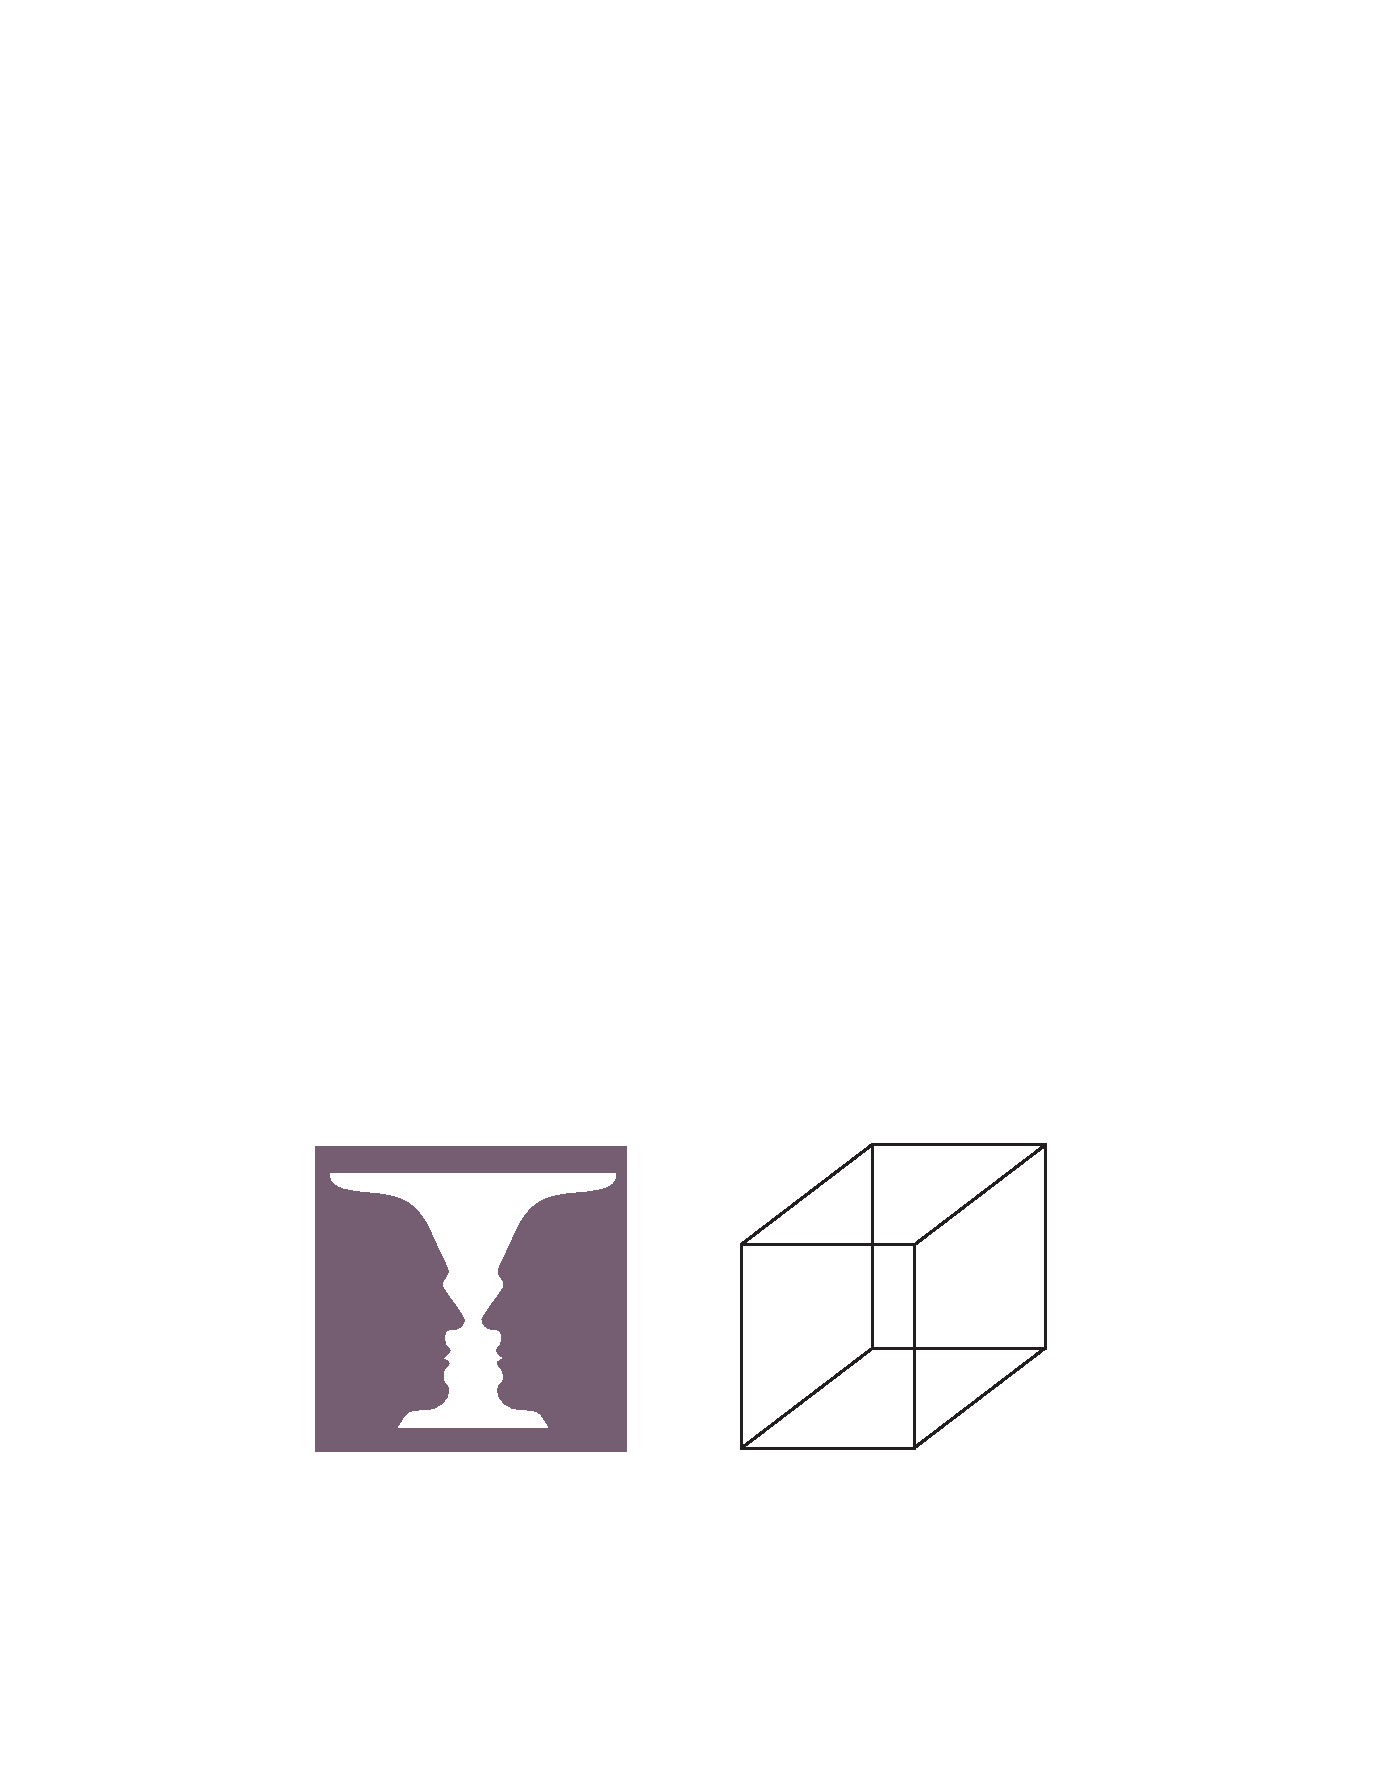
\includegraphics[width=0.7\linewidth]{chap59/fig_59_2}
	\caption{模棱两可的数字。 如果你盯着左边的人物(鲁宾人物),你有时会看到一个花瓶,有时会看到两张面孔。 如果你盯着右边的图(内克立方体),你会看到一个三维立方体,但立方体的正面有时会出现在左下角,有时会出现在右上角。 在每个图形中,大脑都会找到两个同样好的但相互排斥的解释。 我们的意识感知自发地在这两种解释之间交替。}
	\label{fig:59_2}
\end{figure}


为了证明变化失明,构建了一个复杂场景的两个版本。
在 Ron Rensink 开发的一个著名示例中,图片由一架停在机场跑道上的军用运输机组成。
在这两个版本之一中,缺少引擎。
如果这两张图片在计算机屏幕上交替显示,但严重地穿插着空白屏幕,即使指出时立即很明显,也可能需要几分钟才能注意到差异。
(另一个示例参见图 25-8。)


鉴于这些现象,我们可以探索当感觉刺激没有变化时与知觉变化相关的神经活动。
同样,我们可以发现感官输入的变化是否在大脑中记录下来,即使没有在意识中表现出来。
我们可以问,与有意识过程相关的神经活动与无意识过程相关的神经活动之间是否存在一些质的差异。


对与特定类型的意识知觉相关的神经活动的研究得出了两个重要结果。
首先,某些类型的知觉与大脑特定区域的神经活动有关。
当有意识地感知物体或特征时,那些专门用于识别某些种类的物体(例如,面部、文字、风景)或某些视觉特征(例如,颜色、运动)的大脑区域会更加活跃(图 59- 3)。
例如,当我们感知鲁宾图中的人脸时,专门处理人脸的梭状回区域活动较多。


这种观察也适用于异常感知(幻觉)。
在导致失明的周围视觉系统退化后,一些患者会出现间歇性幻视(Charles Bonnet 综合征)。
这些幻觉因患者而异:一些患者看到彩色斑块,其他患者看到网格状图案,有些甚至看到面孔。
Dominic ffytche 发现这些幻觉与次级视觉皮层的活动增加有关,幻觉的内容与特定的活动部位有关(图 \ref{fig:59_4})。
精神分裂症患者经常会出现复杂的幻听,通常表现为与患者交谈或谈论患者的声音。
这些幻觉与听觉皮层的活动有关。


\begin{figure}[htbp]
	\centering
	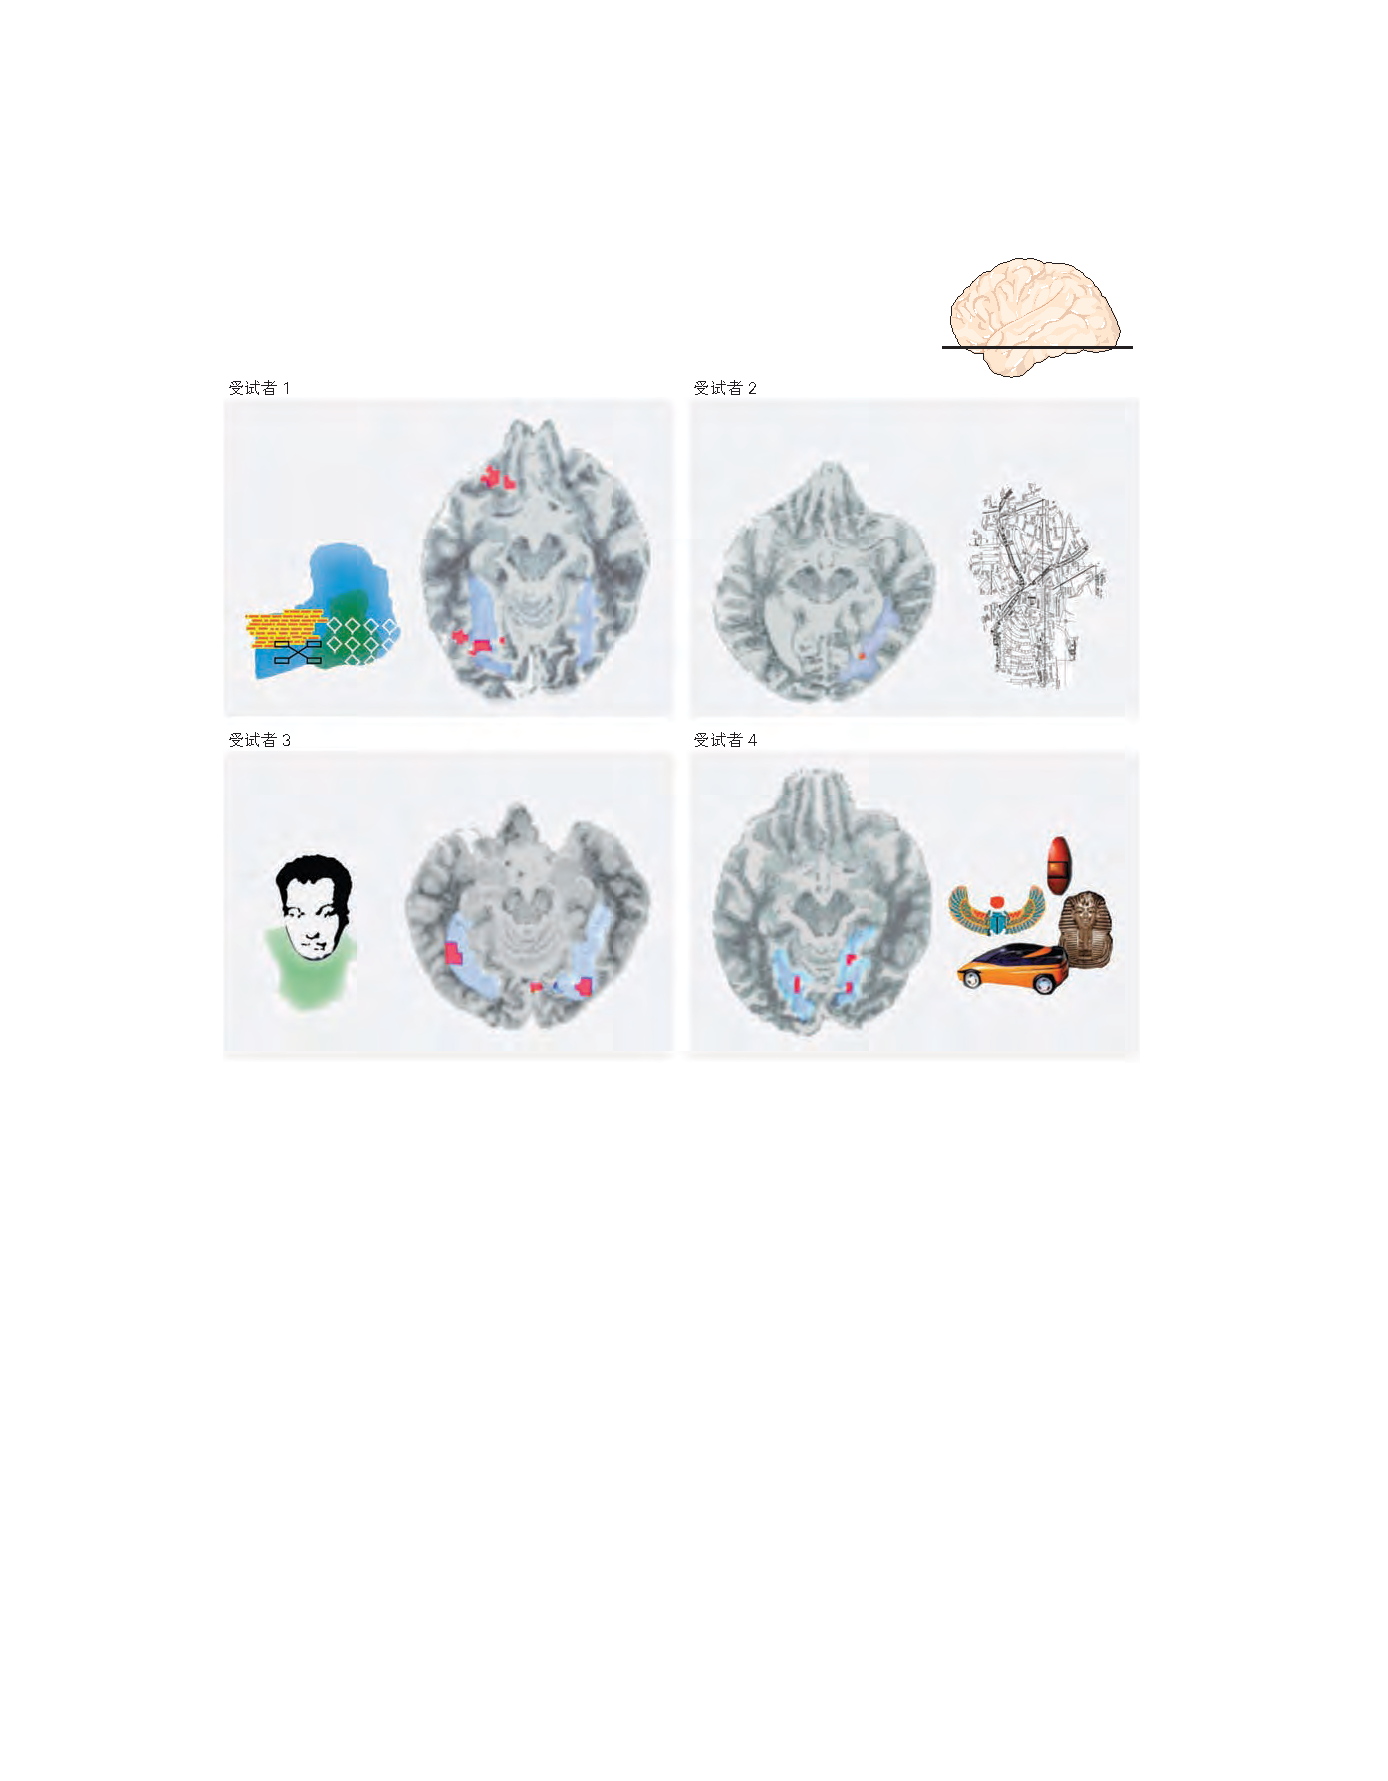
\includegraphics[width=0.8\linewidth]{chap59/fig_59_4}
	\caption{与视觉幻觉相关的神经活动。 一些视网膜受损的患者会出现幻视。 神经活动的位置与幻觉的内容有关。 颜色、图案、物体或面孔的体验与下颞叶皮层特定区域的活动增强(红色)有关。 蓝色区域是梭状回。 (经许可转载自 ffytche 等人,1998 年。版权所有 © 1998 Springer Nature。)}
	\label{fig:59_4}
\end{figure}


这些观察结果表明,有意识的体验可能源于某些皮层区域的活动。
这个想法很难通过实验检验,但在 1950 年代,神经外科医生 Wilder Penfield 发现,对接受神经外科手术的患者的皮层进行电刺激可以产生有意识的体验。
最近,已经发现对 V5/MT 区域的皮层进行经颅磁刺激可以导致看到移动的闪光。


从试图将神经活动与特定知觉相关联的研究中得出的第二个重要结论是,专门领域的活动是必要的,但不足以产生有意识的体验。
例如,在变化盲范式中,受试者通常不会意识到他们正在查看的图片发生了巨大变化。
如果变化涉及面部,则无论受试者是否意识到变化,梭状回都会引起活动。
但是,当感觉变化也被有意识地感知到时,顶叶和额叶皮层就会另外活动(图 \ref{fig:59_5})。


\begin{figure}[htbp]
	\centering
	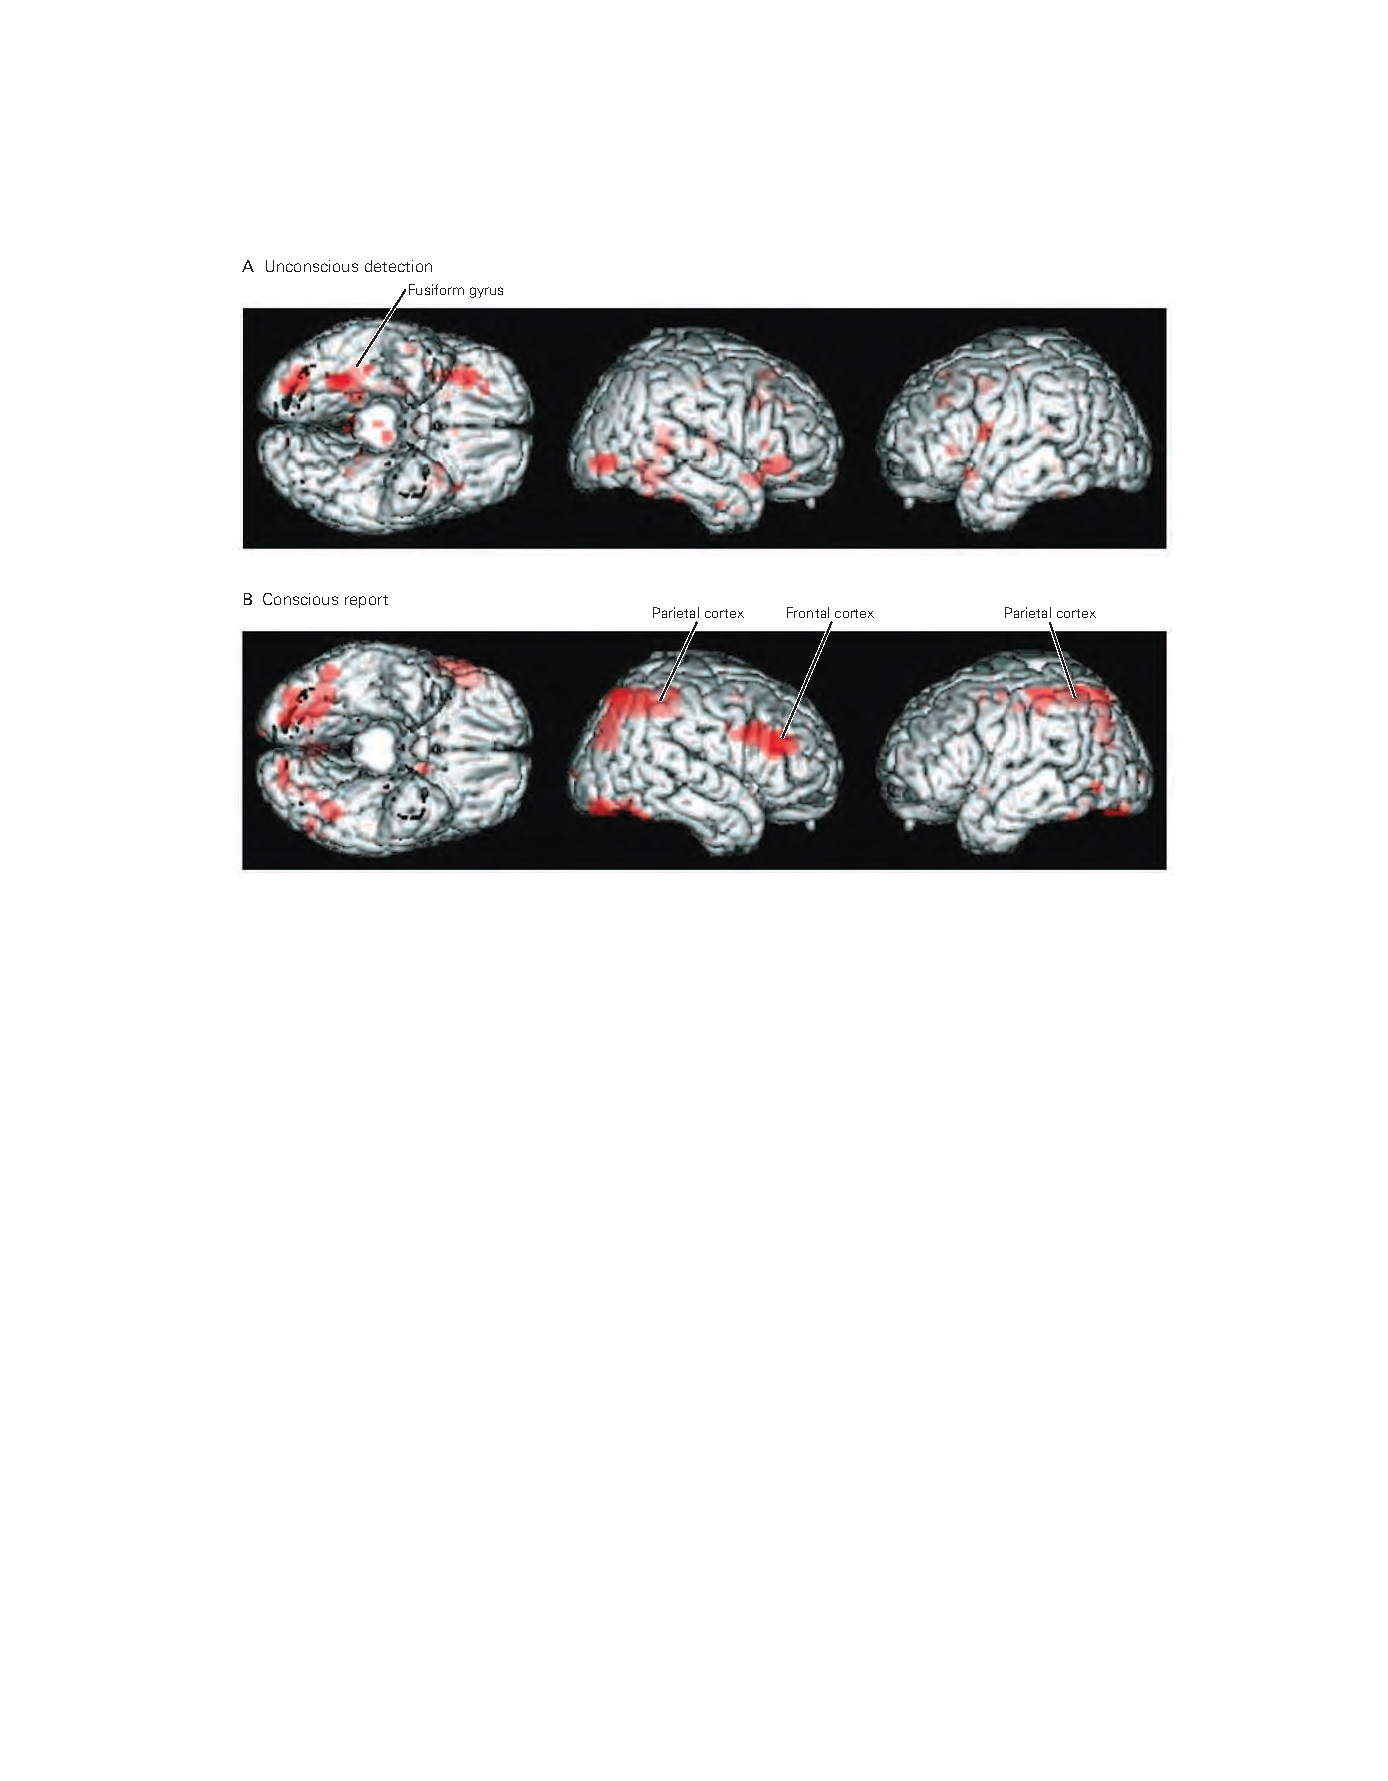
\includegraphics[width=0.8\linewidth]{chap59/fig_59_5}
	\caption{有意识和无意识的大脑活动。 当受试者看到的面部发生变化时,梭形面部区域的活动会增加,无论受试者是否意识到或意识到这种变化。 当受试者意识到这种变化时,顶叶和额叶皮层的活动也会增加。 (经许可转载自 Beck 等人,2001 年。)}
	\label{fig:59_5}
\end{figure}


这些观察与我们对单方面忽视的理解有关。
由于左侧的物体仍然会在视觉皮层中引起神经活动,因此右侧顶叶皮层的损伤可能只是阻止了对空间左侧物体的有意识表征的形成。
然而,这种感觉活动可以支持患者的无意识推断,即他们不想住在左侧燃烧的房子里。


没有进入意识的刺激也可以引起明显的反应。
一张带有恐惧表情的脸会在自主神经系统中引起恐惧反应,表现为出汗导致的皮肤电导(电流反应)增加。
即使面部紧随其后是另一个视觉刺激,这种反应也会发生,这样面部就不会被有意识地感知到。
拥有快速但分辨率低的系统来识别危险事物可能会有优势。
我们先跳;
只是后来,在一个缓慢的高分辨率系统的基础上,我们才能够识别出让我们跳跃的物体(第 \ref{chap:chap48} 章)。
这两个识别系统中的一个或另一个的损坏可以解释某些令人费解的神经和精神疾病。


面容失认症是一种知觉障碍,面孔无法辨认。
病人知道他在看一张脸,但无法认出那张脸,即使是一张熟悉多年的心爱的脸。
这个问题是面部特有的,因为患者可能仍然能够从他们的衣服、步态和声音中认出这个人。
然而,面容失认症患者能够在不知不觉中识别面孔。
他们对熟悉的面孔表现出自主反应,并且在被要求猜测展示给他们的面孔是否属于熟悉的人时,他们比凭运气做出更好的反应。
事实上,他们对一张脸引起的自主(情绪)反应的意识可能使他们能够判断熟悉程度。


Capgras 综合症是一种错觉,偶尔会在精神分裂症患者和一些脑损伤或痴呆症患者身上观察到,它会产生更令人不安的体验。
这些患者坚信他们身边的某个人,通常是丈夫或妻子,已经被冒名顶替者所取代。
他们声称这个人虽然外表相似但不完全相同,但实际上是另一个人。
通常,这种错觉是在要求冒名顶替者离开房子的情况下产生的。


Hadyn Ellis 和 Andy Young 认为这种奇怪的错觉是面容失认症的镜像现象。
根据这种观点,面部识别回路是完整的,但调解对面部的情绪反应的电路却不是。
结果,患者认出了眼前的人,但由于缺乏情绪反应,觉得有根本的问题。
这些患者对熟悉的面孔没有正常的自主反应的观察结果部分证实了这一说法。


这种解释意味着 Capgras 错觉不是思维混乱的结果,而是经验混乱的结果。
一个病人看到他妻子的脸时没有正常的情绪反应。
这不是他的妻子而是冒名顶替者的结论是对这种异常经历的认知反应,是大脑试图解释这种经历的尝试。


\section{行动的控制在很大程度上是无意识的}

我们可以控制自己的行为的感觉是意识的主要组成部分。 但是我们是否了解自己行为的所有方面?
大卫·米尔纳 (David Milner) 和梅尔·古德尔 (Mel Goodale) 研究了一位名叫 D.F. 谁表现出对自己行为的某些方面明显缺乏认识。
由于一氧化碳中毒导致她的下颞叶受损,D.F. 患有形式失认症——她无法识别事物的形状。
她无法区分正方形和长方形卡片,也无法描述插槽的方向。
然而,当她拿起长方形卡片将其放入槽中时,由于视觉运动回路的无意识操作,她会调整手的方向并适当地握住手(图\ref{fig:59_6})。


\begin{figure}[htbp]
	\centering
	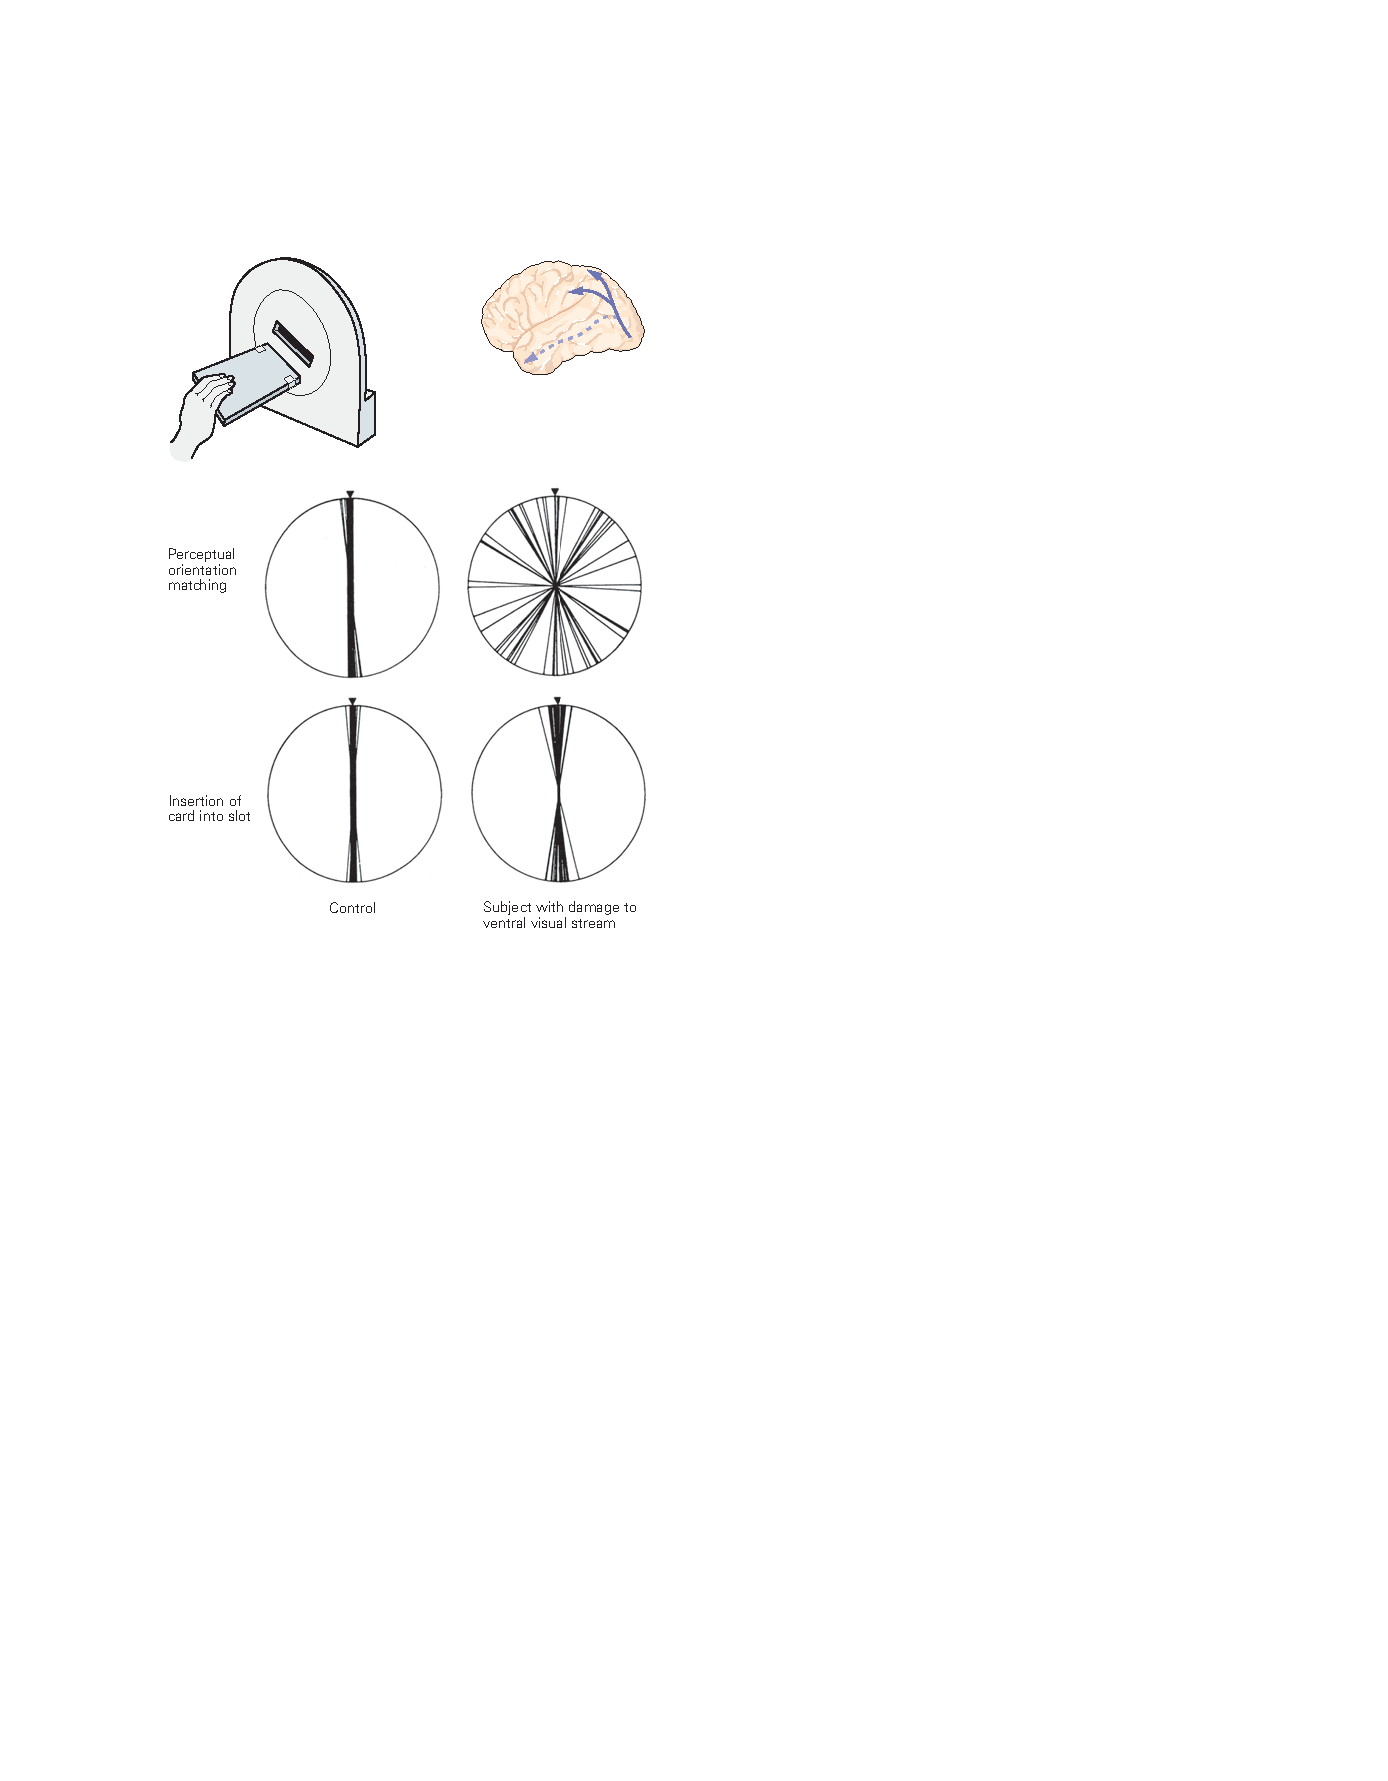
\includegraphics[width=0.5\linewidth]{chap59/fig_59_6}
	\caption{行动可以通过无意识的刺激来控制。 下颞叶皮层受损的患者 D.F. 无法根据物体的形状识别物体(形成失认症)。 她无法将平板电脑与插槽的方向对齐(感知匹配),因为她没有意识到平板电脑或插槽的方向。 然而,当她被要求快速将平板电脑穿过插槽时,她会快速准确地调整手的方向。 据推测,运动是由受试者不知道的视觉运动计算驱动的。 (经许可改编自 Milner 和 Goodale 1995。)}
	\label{fig:59_6}
\end{figure}


这种无意识的引导并不是脑损伤患者独有的。
在 D.F. 因为通常将有关形状的视觉信息带入意识的系统受损了。
事实上,我们都可以做出快速准确的抓握动作,而无需意识到用于控制这些动作的知觉和运动信息。
有时,我们甚至没有意识到自己做了动作。
这种用于视觉引导的伸手和抓取的很大程度上是无意识的系统类似于与恐惧反应相关的快速但分辨率低的系统,并且可能与之重叠。


虽然我们可能没有意识到诸如伸手和抓握等动作的感知和运动细节,但我们清楚地意识到我们可以控制我们的某些行为——我们意识到我们引起的行为与非自愿发生的行为之间的区别。
本杰明·里贝特研究了受控实验中的自愿行为现象。
他要求他的受试者“每当他们感到有这样做的冲动时”就举起一根手指,并报告他们产生这种冲动的时间。
他的受试者在可靠地报告这种主观体验的时间方面没有困难。
与此同时,利贝特使用脑电图来测量“准备潜力”,这是一种大脑活动的变化,发生在受试者做出任何自主运动之前最多 1 秒。
受试者报告感到有抬起手指的冲动的时间发生在这种准备潜力开始后数百毫秒。
这一结果在哲学家和神经科学家之间引起了很多关于自由意志存在的讨论。
如果大脑活动可以在一个人意识到有执行该动作的冲动之前预测该动作,这是否意味着我们对自由意志动作的体验是一种错觉?


尽管 Libet 的结果已被广泛复制,但他的实验方案对我们理解自由意志的相关性仍存在争议。
举起一根手指不是我们经常执行的动作。 行动通常有目标。
例如,我们可能会按一个按钮来响铃。
当我们的行动遵循我们期望的目标时,我们会觉得我们可以控制自己的行动。
正是这种主观体验给了我们一种能动性,成为事件的起因。
将 Libet 的范式应用于此类行为,Patrick Haggard 发现了“故意绑定”现象。
当一个有意的动作(按下一个按钮)之后是它的预期目标(听到一个音调)时,这些事件在主观上被体验为在时间上绑定在一起(图 \ref{fig:59_7})。


\begin{figure}[htbp]
	\centering
	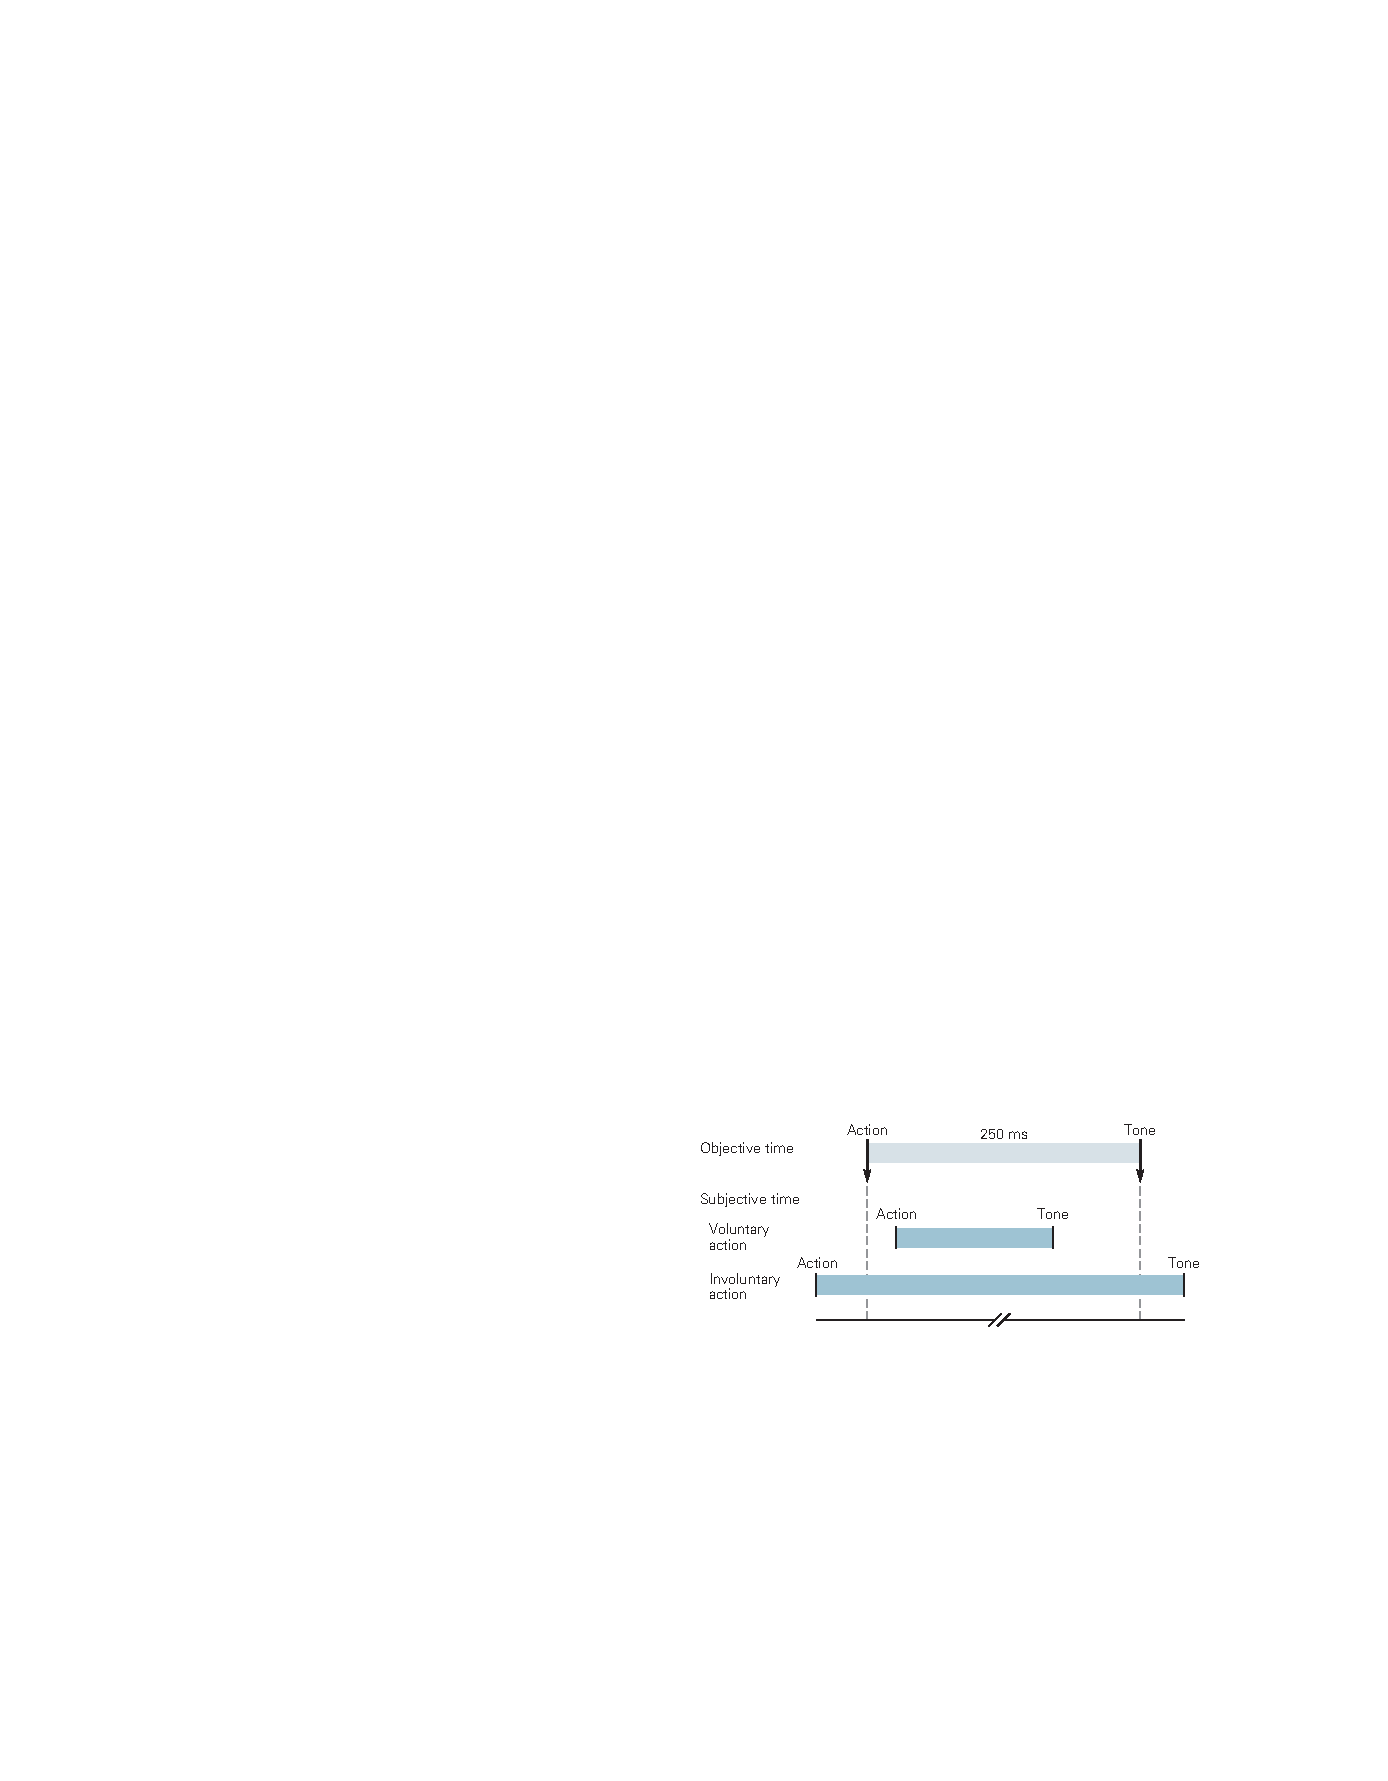
\includegraphics[width=0.5\linewidth]{chap59/fig_59_7}
	\caption{我们体验到我们的行为和它们的影响是及时结合在一起的。 当要求受试者在 250 毫秒后按下触发声音的按钮时,他们会体验到他们的动作和声音的发生时间(主观时间)比实际情况(客观时间)更近。 相比之下,当他们的手指通过运动皮层的经颅磁刺激 (TMS) 不由自主地移动时,与客观时间相比,运动和声音会感觉更远。 时间约束只有在运动是有意和深思熟虑时才会发生,因此是代理体验的标志。 (基于 Haggard、Clark 和 Kalogeras 2002。)}
	\label{fig:59_7}
\end{figure}


我们的行动与他们的目标的这种时间绑定为我们的代理感提供了一个经验标记,因为更强的代理感与更大程度的绑定相关联。
如果运动是被动发生的,例如由对大脑的磁刺激引起,那么有意的束缚就会减少;
我们实际上认为运动和结果之间的时间比实际的物理时间要长。


我们的代理意识与我们对自由意志的信念以及人们在故意执行这些行为时可以对他们的行为负责的想法密切相关。 当与具有道德后果的结果相关联时,故意约束力会增加。
它减少了其他人命令的动作,而不是自由执行的动作。
这些结果并没有解决自由意志是否存在的问题,但它们表明我们自由行动的有意识体验在创造社会责任规范方面起着重要作用。
这些规范对于维持社会凝聚力至关重要。


无意识推理发生在运动领域和感觉领域。
我们的代理体验由两个部分组成:我们先前的期望和行动结果的感官后果。
如果实际感觉与我们的预期不符,我们会感到惊讶,例如当我们拿起一个比预期轻得多的物体时(第 \ref{chap:chap30} 章)。
然而,如果结果证实了我们的预期,我们就会很少注意实际的感官证据——我们会体验到我们预期会发生的事情,而不是实际发生的事情。


Pierre Fourneret 和 Marc Jeannerod 要求受试者使用电脑鼠标画一条垂直线。
受试者看不到他们的手,因此看不到计算机在屏幕上显示的线条中造成的扭曲。
惊人的结果是受试者没有意识到他们将手向左移动 10° 角以在屏幕上产生垂直线(图 \ref{fig:59_8})。
这种意识的缺乏发生在高达 15° 的偏差中。
当受试者被指示不要看屏幕而只是重复他们刚刚做过的动作时,他们并没有重现他们做过的异常动作,而是画出他们认为自己做过的笔直向前的动作。
似乎只要实现了目标(画一条直截了当的线),我们就会体验到预期的感官反馈,而不是实际的感官反馈。


\begin{figure}[htbp]
	\centering
	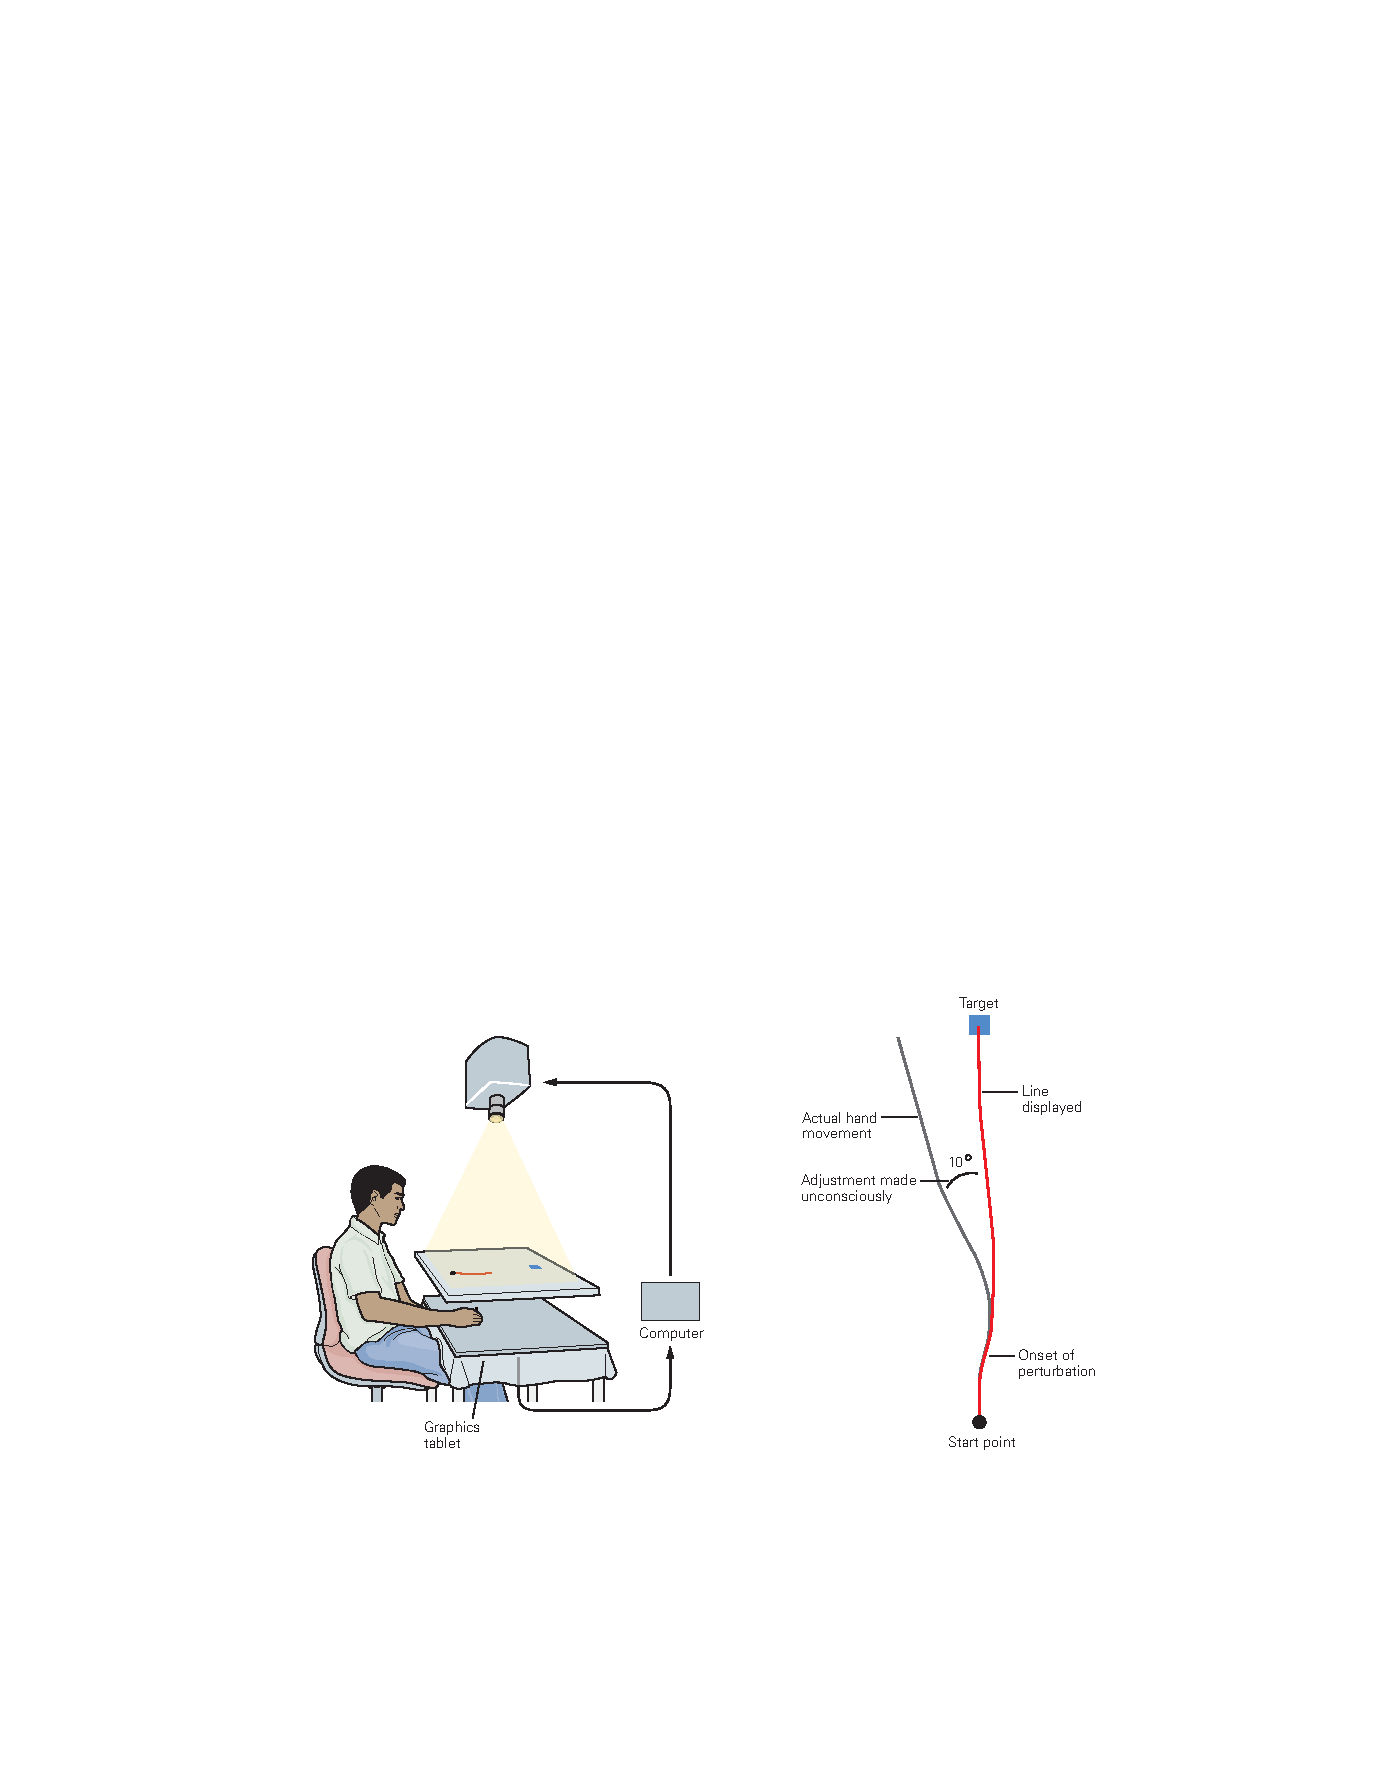
\includegraphics[width=0.65\linewidth]{chap59/fig_59_8}
	\caption{可以在不知不觉中修改动作。 受试者被要求用电脑鼠标画一条直线。 他们可以看到屏幕上的线条,但看不到他们的手部动作。 计算机被编程为系统地扭曲屏幕上显示的线条。 在这里显示的结果中,受试者必须将他的手向左移动 10°,以在屏幕上产生一条垂直线。 对象并不知道做出这样的调整。 (经许可改编自 Fourneret 和 Jeannerod 1998。版权所有 © 1998 Elsevier Science Ltd.)}
	\label{fig:59_8}
\end{figure}


这种现象有助于我们理解一些原本奇怪的经历。
例如,在肢体截肢后,一些患者可能会出现幻肢。
他们仍然有移动缺失肢体的冲动,并且可以选择希望缺失肢体进行的特定动作。
他们的感觉运动系统预测如果他们要移动一个完整的肢体他们会感觉到的本体感觉,而正是这些预测的感觉构成了移动幻肢感觉的基础。


在肢体因中风而瘫痪后,一些患者认为他们仍然能够移动肢体(偏瘫的失认症)。
同样,在这里,这些患者可以选择他们想要进行的动作,并了解他们对动作的期望。
尽管在他们尝试开始运动后缺乏感官证据,但他们相信运动确实发生了。



\section{有意识地回忆记忆是一个创造性的过程}

对于我们大多数人来说,记忆是对过去经历的有意识的想象重温。
然而,如果我们不考虑主观经验(行为主义立场),记忆就是我们过去的经验改变未来行为的过程。
我们的行为通常会受到过去经验的影响,但不会有意识地回忆记忆或意识到它对我们的影响。
再一次,这种类型的体验在大脑特定区域受损的患者身上最为明显。


一些患者在颞叶内侧区域受损后变得严重遗忘。
根据智商测试,他们的智力没有下降,但在几分钟内什么都记不住。
尽管具有破坏性,但这种记忆障碍实际上是相当有限的。
这个问题主要体现在陈述性记忆中,最严重的是一种称为情景记忆的陈述性记忆,即回忆生活中事件的能力(第 \ref{chap:chap54} 章)。
意识在其中起次要作用(第 \ref{chap:chap53} 章)的程序性记忆保持完好。
因此,患者仍然可以记住骑自行车等运动技能,并且通常可以正常速度学习新的运动技能。
脑损伤的这种选择性作用会导致剧烈的解离。
每周都在学习一些新技能的患者会否认以前曾执行过这项任务。
然后他惊讶地发现自己变得如此熟练。


一项广泛使用的协议测试了受试者回忆起他们所记住的单词列表的能力,这是一项利用陈述性记忆形式的任务。
在回忆阶段,受试者会看到学习列表中的单词列表以及新单词。
健忘症患者很难完成此类任务,并且可能会将大部分以前见过的单词错误归类为新单词,因为她不记得以前见过它们。
然而,阅读旧词引发的大脑活动与新词引发的不同:
存在对差异的无意识识别,相当于单侧忽视或面容失认症患者表现出的差异。
普通受试者通常会发现这项任务很容易,但他们偶尔也会将旧词错误分类为新词;
与健忘症患者一样,在正常受试者中诱发的大脑反应记录了有意识回忆所失去的区别(图 \ref{fig:59_9})。


\begin{figure}[htbp]
	\centering
	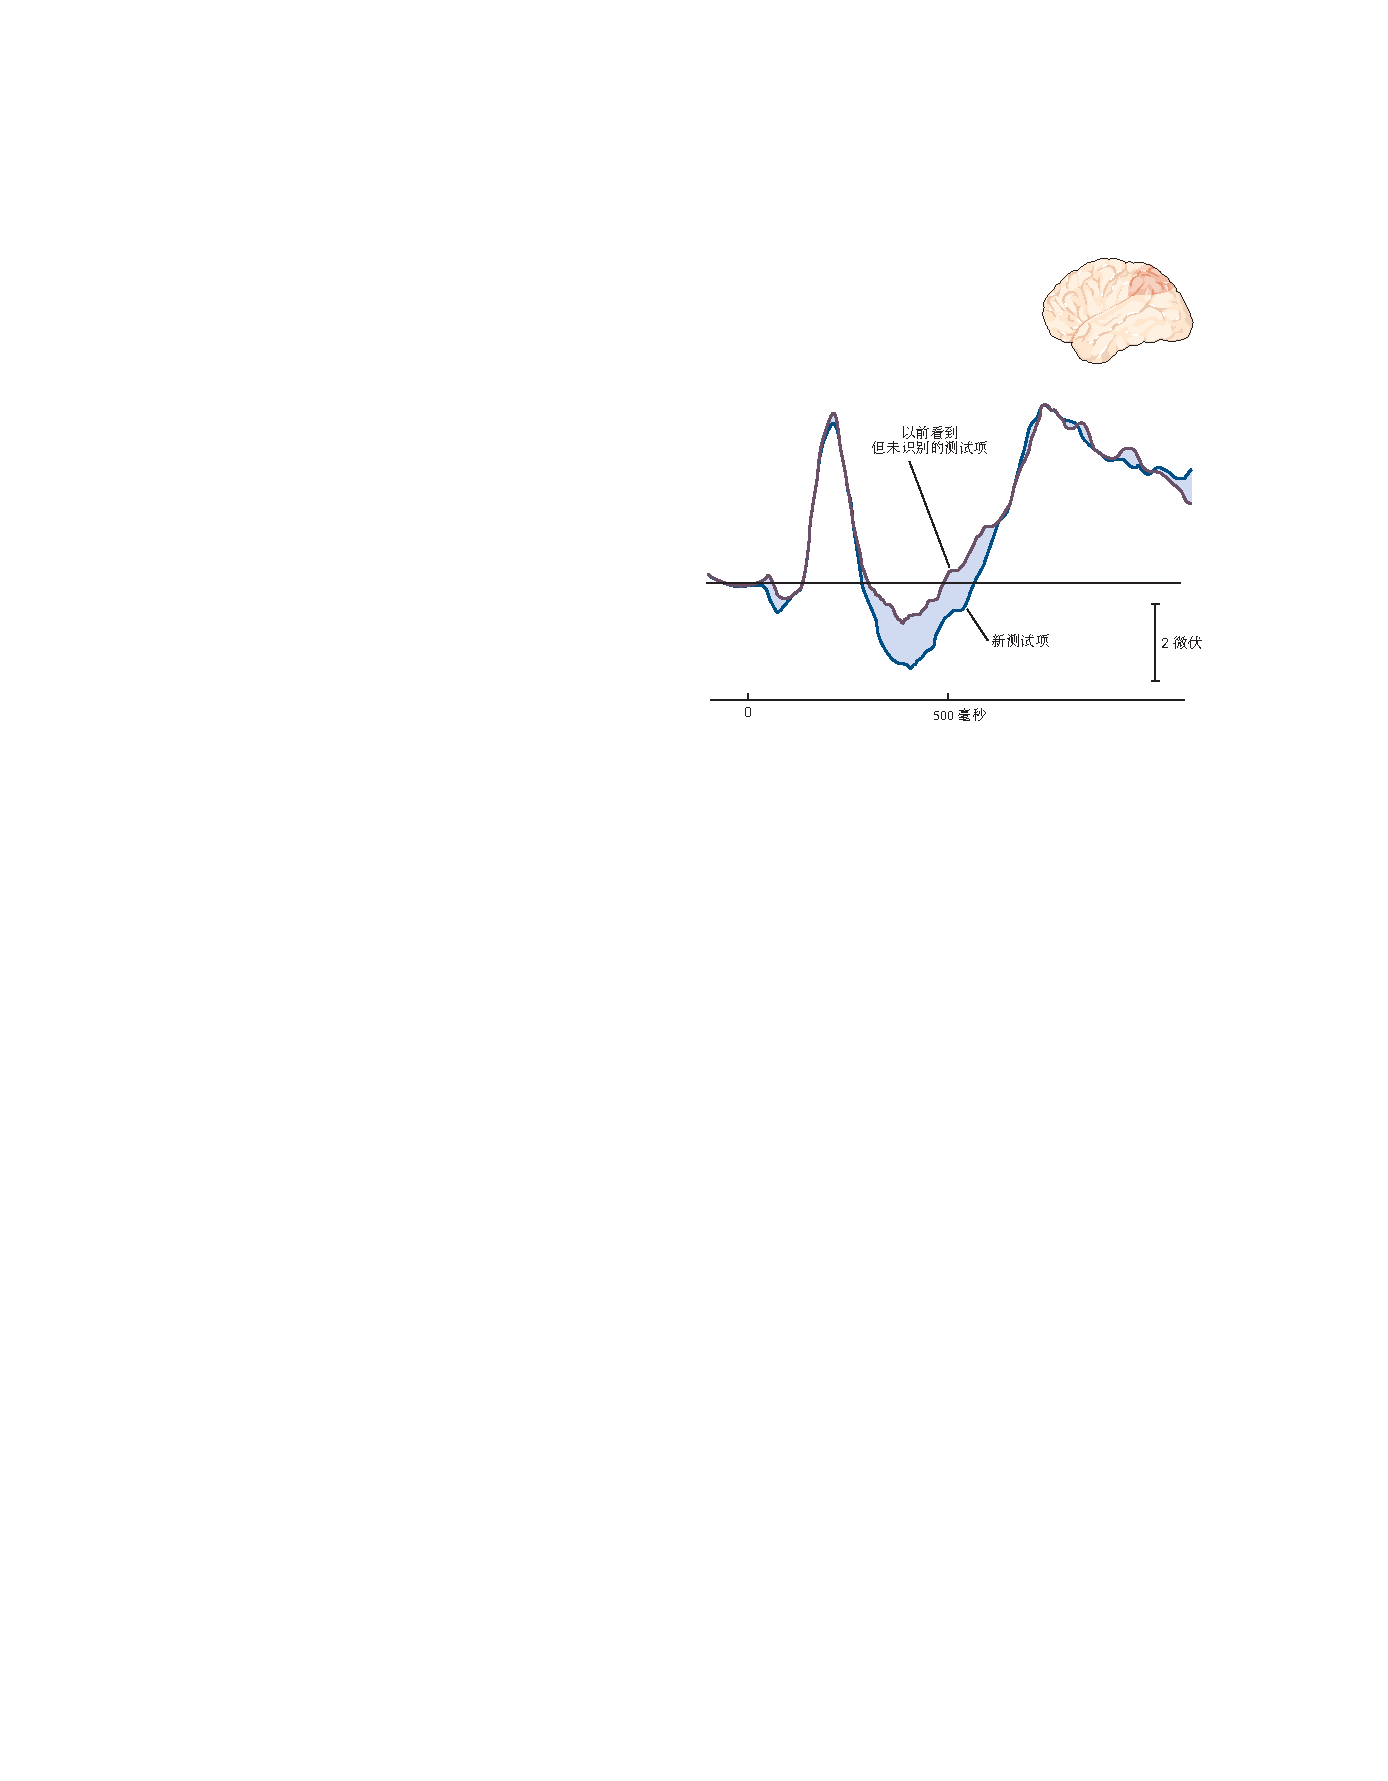
\includegraphics[width=0.5\linewidth]{chap59/fig_59_9}
	\caption{大脑活动显示被遗忘记忆的印记。 向受试者展示了一个单词列表,其中包括一些较早出现的单词和一些新单词。 当被要求识别之前出现的单词时,受试者正确识别了一些旧单词但忘记了其他单词。 在一个词的视觉呈现之后,大脑中的诱发电位会立即出现短暂的波动。 大脑顶叶区域的诱发反应反映了这些词是否以前见过,即使受试者没有有意识地认出这些词。 旧词产生的模式,无论是否被识别,都与新词产生的模式不同。 (经许可转载自 Rugg 等人,1998 年。版权所有 © 1998 Springer Nature。)}
	\label{fig:59_9}
\end{figure}


有时,受试者会将新词错误分类为旧词。
这种错误分类相当于错误的记忆。
当新词与一个或多个旧词在语义上相关时,最有可能发生这种错误分类。
如果旧词列表包含 big、great、huge,那么新词 large 很可能被识别为 old。
对此的一种解释是,对新词 large 的感知已经在不知不觉中被先前出现的旧词所激发。
因此,新词 large 的处理变得容易且快速,并且因为受试者意识到了这一点,所以他断定这个词一定很熟悉,并将其归类为旧词。


这一观察强调记忆是一个创造性的过程。
我们有意识的记忆是由有意识的回忆和无意识的知识构成的。
为了防止错误的记忆,就像错误的知觉一样,我们利用我们对世界的了解来确定哪些记忆是可信的。


在某些患者中,筛选记忆的过程会变得非常混乱。
如果被问到昨天发生了什么,大多数健忘症患者会说他们不记得了,但也有少数人会详细描述与事实不符的情况。
这种错误的记忆被称为虚构,有时非常难以置信。
例如,一名患者说他见过哈罗德·威尔逊(英国前首相),并讨论了他们正在从事的一项建筑工作。


在想象未来可能发生的事件时,还涉及重建过去情节记忆所需的创造性机制。
在海马体受损的健忘症患者中,想象新事件的能力明显受损。



\section{行为观察需辅以主观报告}

到 20 世纪中叶,经典的行为主义方法显然不足以探索许多心理过程。
语言习得、选择性注意和工作记忆不能根据刺激和反应之间的关系来理解,无论假设的关系多么复杂。


证明某些认知过程是无意识的需要我们进一步远离行为主义。
如果我们想探索整个范围的有意识和无意识的认知过程,我们将无法仅通过关注外显行为来做到这一点。
我们不能假设一个主体做出有目的的、以目标为导向的行为一定会意识到引发该行为的刺激,甚至是该行为本身。
我们必须用主观报告来补充行为观察。
我们必须问受试者,“你看到刺激了吗? 你的手动了吗?”


一百年前,内省是获取心理学数据的主要方法。
否则如何研究意识?
但是不同的心理学流派得到了不同的结果,而且正如约翰·B·沃森所强调的那样,似乎没有客观的方法来决定谁是对的。
您如何独立确认主观体验?
因此,该方法声名狼藉。 在行为主义主导心理学的几十年里,主观报告不被认为是合适的数据来源。
因此,记录主观报告的方法远远落后于记录公开行为的方法。
遗憾的是,许多认知过程研究仍然不需要受试者的主观体验报告,因为长期以来一直有排除此类报告的传统。


继续使用主观报告的一个心理学领域是心理物理学,费希纳于 1860 年引入了对感觉(身体能量)和知觉(心理体验)之间关系的研究。这些研究给出了稳健可靠的结果,并创造了一些 心理学中为数不多的定律,例如韦伯定律(两种刺激之间最明显的差异与刺激的大小成正比)。
在这些研究中,受试者通常会被问到“你看到刺激了吗?” 或“您对看到刺激有多大信心?”


信号检测理论于 1950 年代发展起来,它提供了一种可靠的方法来衡量独立于任何报告偏差(第 \ref{chap:chap17} 章)检测刺激的能力(辨别力,d')。
如果您的辨别能力很高,那么您将成功地检测到刺激的微小变化。
最近,人们对第二个问题越来越感兴趣,“你对看到刺激措施有多自信?” 
报告一个人的信心需要元认知,即反思我们的认知过程的能力。
这种能力对行为的控制有重要作用。
例如,如果我们意识到我们没有很好地执行某项任务,我们可能会放慢速度并更加注意我们正在做的事情。


可以客观地衡量反思我们感知的能力。
同样,也可以定量评估反思我们认知过程质量的能力。
如果你的元认知准确性很高,那么你将成功地区分正确和错误的答案。
换句话说,正确的检测通常与高置信度相关联,而不正确的检测与低置信度相关联。
但是,您的元认知准确性不一定与您的信号检测能力相关。
您可能擅长检测信号,但同时却不太了解您的答案可能是对还是错。
事实上,前额叶皮质受损的患者保留了检测视觉信号的能力,但在元认知准确性方面表现出明显的缺陷。


当然,口头报告不能用于实验室动物或不会说话的婴儿的信号检测实验。
一种替代方法是确定反映信心的行为的各个方面。
例如,如果我们确信我们把钥匙落在了客厅的某个地方,我们就会在切换到大厅之前花更多的时间寻找那里。
Louise Goupil 和 Sid Kouider 将这一见解应用于学前婴儿的元认知研究。
婴儿必须记住两个盒子中的哪一个装有玩具,后来在他们不知情的情况下将其拿走了。
他们花了更多时间在正确的盒子里搜索。
婴儿也更有可能向成人寻求帮助以打开正确的盒子。
这些影响在长时间间隔后不会发生。
这种行为表明婴儿对他们当前的知识状态有一些了解。
他们知道什么时候他们不再记得哪个是正确的盒子。
类似的实验表明,老鼠和猴子也有一些元认知能力。



\subsection{主观报告的验证具有挑战性}

主观经验的报告,例如信心,就像一个仪表。
正如电表将电阻转换为表盘上指针的位置(读数为 100 欧姆)一样,受试者将光刺激转换为颜色报告(“我看到红色”)。
但有一个关键的方法,就是计不似人。
仪表不会遇到红色,也无法传达意义。
而且,尽管仪表可能有故障,但它绝不会在真正看到蓝色时假装看到红色。
大多数时候,我们假设主观报告是真实的,也就是说,受试者正在尽可能准确地描述他的经历。
但是我们如何确定我们可以依赖这些主观报告呢?


使用脑成像可以部分解决验证主观报告的问题。
大脑成像研究表明,在与任何明显行为无关的心理活动期间,神经活动发生在大脑的局部区域。
这种心理活动的内容,如想象或白日梦,只能从受试者的报告中获知。


如果我们扫描一个对象,而他说他正在想象移动他的手,则会在运动系统的许多部分检测到活动。
在大多数运动区域,这项活动的强度低于与实际运动相关的活动,但远高于静息水平。
同样,如果受试者报告说她正在想象她最近看到的一张脸,则可以在梭状回(“面部识别区域”)中检测到活动(图 \ref{fig:59_10})。
在这些示例中,扫描仪检测到的观察到的神经活动的位置提供了对主体报告的体验内容的独立确认。
在某些有限的情况下,意识的内容可以从神经活动的模式中推断出来。


\begin{figure}[htbp]
	\centering
	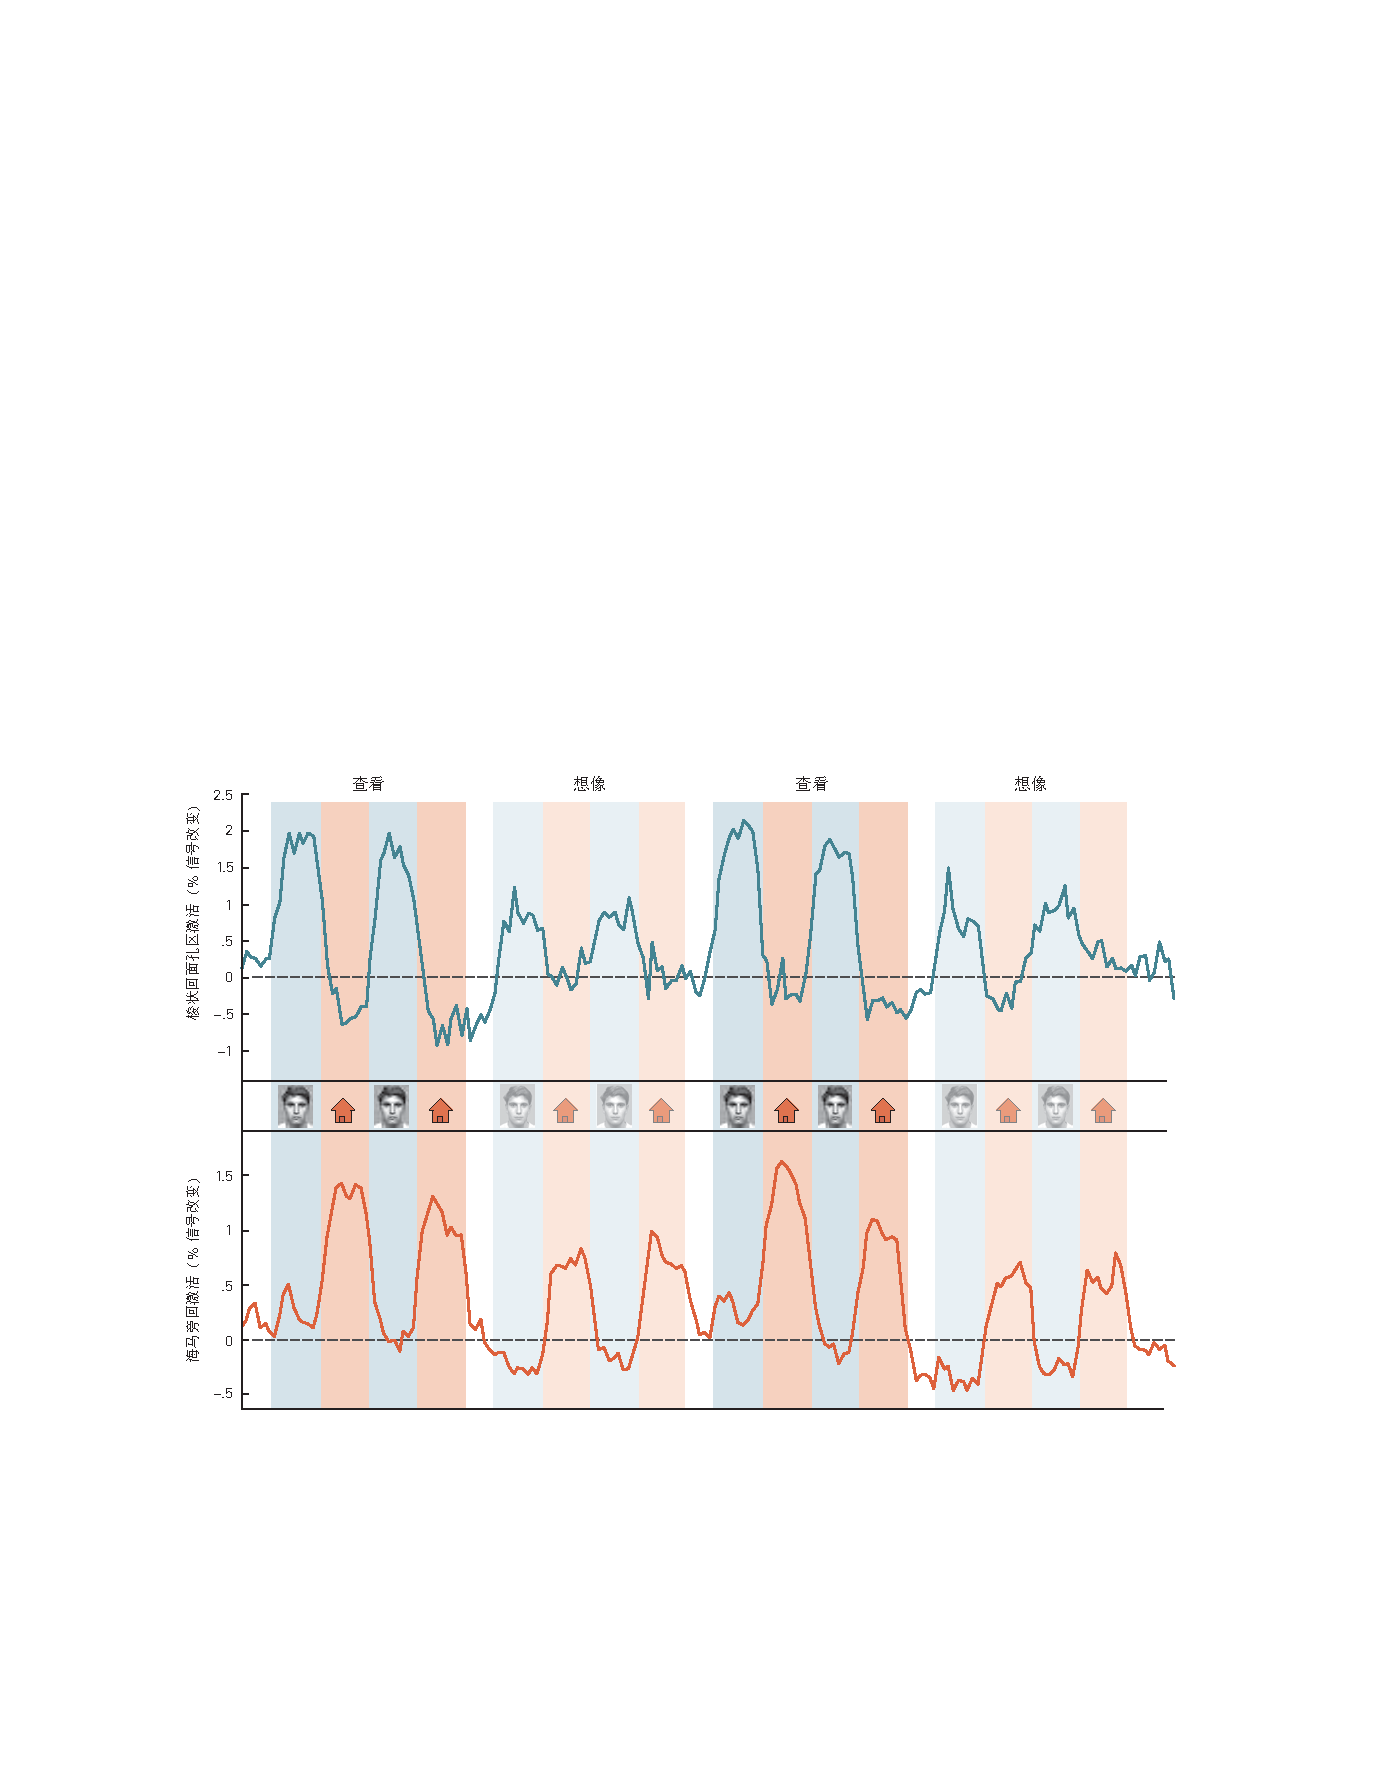
\includegraphics[width=0.9\linewidth]{chap59/fig_59_10}
	\caption{想象一张脸或一个地方与大脑特定区域的活动相关。 受试者在观看或想象面孔和房屋时被扫描。 在第一组试验中,受试者交替观看一张脸或一座房子。 观看面部时,下颞叶 (FFA) 的梭形面部区域的大脑活动会增加。 在看房子时,下颞叶皮层 (PPA) 的海马旁区域的大脑活动会增加。 在接下来的试验中,受试者交替想象一张脸和一座房子。 在想象和直接观看面孔和房屋时,相同的大脑区域都处于活跃状态,尽管在想象观看时这种活动不太明显。 (经许可转载自 O'Craven 和 Kanwisher 2000。版权所有 © 2000 MIT。)}
	\label{fig:59_10}
\end{figure}



\subsection{装病和歇斯底里会导致不可靠的主观报告}

如果受试者报告说看到“蓝色”,即使他们体验到的是红色怎么办?
怎么会出现这种情况,这种情况下的主观报告情况如何?


考虑一位因内侧颞叶皮层严重受损而失忆的患者。
给病人看一张他每天在病房里见到的人的照片,尽管生理测量(脑电图或皮肤电导)显示对这张照片有反应(但对他没见过的人的照片没有反应),但病人否认曾经见过这个人 前)。
我们的结论是,有意识的记忆过程已被破坏,而无意识的过程则保持完整。
这位病人的主观报告准确地描述了他有意识地知道的事情,但排除了他“知道”的那些没有进入意识的事情。


另一名病人被发现在街上游荡,没有脑损伤的迹象,但报告说他不记得任何关于他自己或他的历史。
当展示他过去的人的照片时,他否认对他们有任何了解,但与此同时,他表现出对照片的生理反应。
在这种情况下,由于缺乏可检测的脑损伤(以及记忆丧失的其他特征),我们开始怀疑他陈述的真实性。
也许生理反应表明他确实有意识地认人。
随后,警方确认了患者的身份,我们发现他因在邻近县犯下严重罪行而被通缉。
我们对他报告的可靠性的怀疑增加了。
最后,当他愚蠢地告诉一位病友:“愚弄那些临床心理学家太容易了。”时,我们的怀疑得到了证实。


在这种情况下,我们有直接证据表明患者故意误导他人对自己的看法。
要欺骗别人,我们不仅要意识到自己的心理状态,还要意识到他人的心理状态。
有什么方法可以测试欺骗吗?
一种方法是使用前面讨论的那种记忆测试。
患者研究单词列表。
然后向他展示一个新列表,其中包含他刚刚学过的单词和新单词,他必须决定每个单词是旧单词还是新单词。
一个真正的健忘症患者不会认出任何一个词;
他将不得不猜测,但通过无意识的启动效应,他会比偶然表现得更好。
装病的病人可以认出这些旧词,但会强烈否认他以前见过它们。
除非他非常老练,否则他的表现可能比碰巧还差。
看来我们应该能够区分真正的健忘症患者和装病者。


第三种病人也假装失忆(或其他一些疾病),但这样做是无意识的,因此不是装病者。
这种情况被称为癔症性或心因性失忆症。
像装病者一样,他在识别测试中的表现比偶然情况更糟。
尽管如此,他并没有意识到他的模拟。
同样的机制发生在被催眠的正常人身上,然后被告知他们对刚刚发生的事情没有记忆。
这种现象有时被称为分离状态:大脑中记录经验和进行口头报告的部分已经与创建模拟的部分分离。
歇斯底里的模拟也会造成感觉丧失,例如歇斯底里性失明和运动障碍,例如歇斯底里性麻痹或歇斯底里性肌张力障碍。


我们距离理解这些疾病的认知过程或潜在生理学还有很长的路要走。
一个关键问题是如何区分歇斯底里和装病。
从意识体验的角度来看,这两种障碍是完全不同的:
装病者意识到自己在假装,而癔症患者则不然。
然而,在这两个案例中,患者的主观报告和外显行为非常相似。
难道没有可以区分这些不同疾病的措施吗?
也许证明这些不同意识状态之间的关键区别的唯一方法是通过神经影像学研究。



\section{亮点}

1. 精神障碍的研究迫使我们面对精神和身体之间的概念鸿沟。
不再可能认为精神障碍有精神原因,而身体障碍有身体原因。


2. 认知神经科学对我们弥合这一差距的尝试产生了重大影响,因为它的描述性语言,即信息处理语言,可以同时应用于心理和神经过程。
信息论和计算机的发展暗示了科学如何解决主观体验如何从物理大脑的活动中产生的问题。


3. 现在很清楚,知觉、行动和记忆是许多平行过程的结果,尽管其中一些过程支持有意识的体验,但大多数发生在意识水平以下。 


4. 当其中一些过程受损而其他过程完好无损时,就会出现显着异常。
一名下颞叶皮层受损的患者 D.F. 不再有意识地意识到物体的形状,因此无法描述它或识别它是什么。
尽管如此,她还是可以将她的手摆成合适的形状来拿起物体。


5. 我们对自己行为的细节知之甚少,但我们清楚地意识到处于控制之中(代理感)。
在极端情况下,这种代理感可能会脱离对行动的控制。
肢体截肢后,许多人会体验到可以活动的幻肢,而在肢体因中风而瘫痪后,一些患者认为他们仍然可以活动肢体。
 

6. 回忆过去不像重放视频。
记忆是一种创造性的过程,它建立在不完美的回忆之上,并填充了常识。
由于丧失了这种创造力,健忘症患者很难想象未来,也很难记住过去。


7. 主观体验是人类生活的重要组成部分。
当我们做出决定时,我们的选择是由我们的行为表明的,但我们对该选择的信心是一种主观体验。
我们可以通过口头报告来研究这样的经历。
对我们选择的信心是元认知的一个例子(即反思我们的认知过程的能力)。
额叶皮层的损伤会损害元认知,同时使决策保持完整。 


8. 口头报告并不总是可靠的。
人们可以假装失忆以逃避法律制裁。
这种装病很难被发现,因为它与歇斯底里性失忆症等疾病非常相似,在这种情况下,患者并没有意识到自己正在模拟这种疾病。
认知神经科学面临的挑战是区分这些情况。

